\section{Approach}
% Explanatory figures

Though the goal of RepVGG is to provide a plain VGG-like CNN architecture, training such an architecture with reasonable depth until convergence is hard. The degradation problem leads to an increase of the training loss curve as deeper layers struggle to learn an implicit identity function once shallower layers have learned an ideal mapping \cite{KaimingHe.2015}. Also very deep plain CNNs make backpropagation difficult as gradients vanish when trying to reach shallower layers. Even if there have been studies to make such plain CNNs converge \cite{LechaoXiao.2018, OyebadeKOyedotun.2020}, accuracy-speed trade-off for plain CNNs remained an open research topic. To avoid the strugggles to train a plain CNN directly, RepVGG uses a structural re-parameterization method to transfer model parameters from a trained ResNet-like architecture to a plain VGG-like architecture that is used for inference. 

\begin{figure}[t]
	\begin{center}
		% \fbox{\rule{0pt}{2in}\rule{0.9\linewidth}{0pt}}
		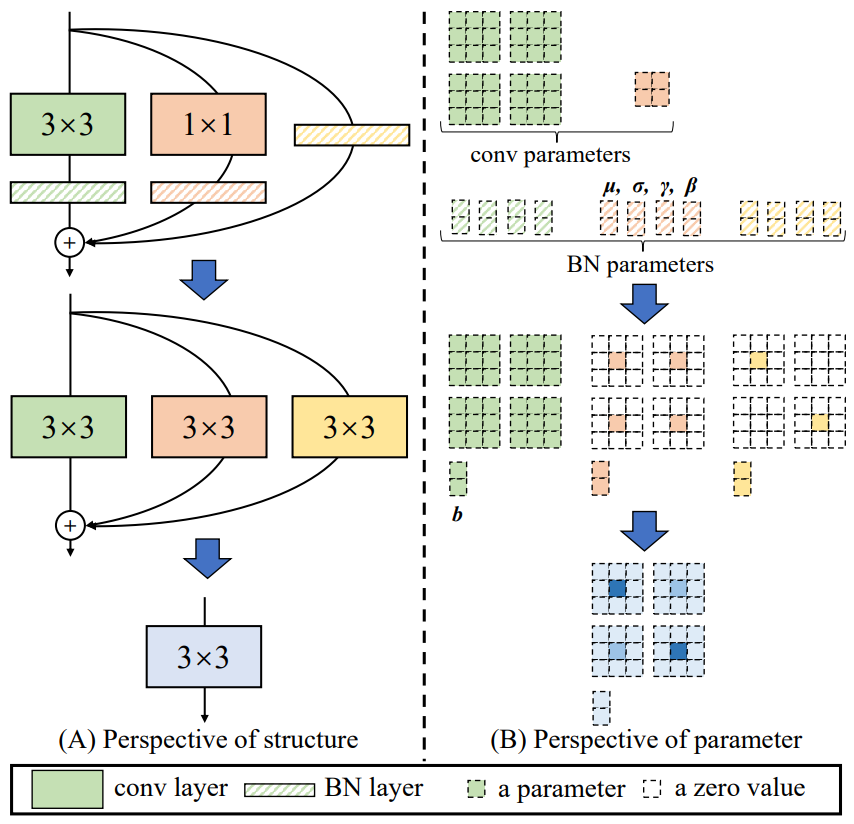
\includegraphics[width=0.8\linewidth]{images/re-parameterization.PNG}
	\end{center}
	\caption{Structural re-parameterization method of RepVGG transforming a 3x3 conv, 1x1 conv and identity branch to a single 3x3 conv layer.}
	\label{fig:reparameterization}
\end{figure}

One layer in the training-time architecture contains three branches, a 3x3 convolution, a 1x1 convolution and an identity branch (see \autoref{fig:reparameterization}). Having the identity branch makes the architecture ResNet-like and prevents the degradation and vanishing gradient problem. The additional 1x1 convolution branch is needed for dimensionality control in case the dimensions would not match when adding the identity skip-connection with the 3x3 convolution branch. In this case the identity branch is omitted. Having such three branches makes the training time model an implicit ensemble of $3^n$ models with $n$ being the number of layers used. 

To transform this layer configuration to a single-path 3x3 convolution simple linear algebra is used. First the identity branch is transformed to a 1x1 convolution using the identity matrix as a kernel. The two 1x1 convolutional layers are then zero-padded to become 3x3 convolutional layers. Next the batch normalization layers need to be transformed. Batch normalization is applied channel-wise to every pixel in a feature map resulting from a convolutional operation of the input channel $M$ with the filter $W$ according to 

\begin{equation} \label{eq:batchnormalization}
	bn(M*W, \mu, \sigma, \gamma, \beta) = (M*W - \mu)\frac{\gamma}{\sigma} + \beta
\end{equation}

with $\mu$ being the accumulated mean, $\sigma$ being the standard deviation, $\gamma$ being the learned scaling factor and $\beta$ being the bias value. One could also realise batch normalization by adapting the convolutional filter and adding a bias value after convolution like 

\begin{equation} \label{eq:batchnormalizationtransformed}
	bn(M*W, \mu, \sigma, \gamma, \beta) = M*(\frac{\gamma}{\sigma}W) - (\frac{\mu\gamma}{\sigma} + \beta).
\end{equation}

To receive the final 3x3 convolutional layer one simple has to add all three kernels together as well as all three bias values (see \autoref{fig:reparameterization}). Note that equal striding as well as compatible padding configurations over the 3x3 and 1x1 branch for the image dimension is necessary to perform such re-parameterization technique. 
